% DO NOT COMPILE THIS FILE DIRECTLY!
% This is included by the other .tex files.

\begin{frame}
\titlepage
\end{frame}

\begin{frame}
  \frametitle{Building a native restSearch export}
  \begin{itemize}
    \item Similar in scope to an export module via MISP modules
    \item Pros:
    \begin{itemize}
      \item Can be used for composited data coming from a search
      \item Fast, native approach
      \item Can be built to support several scopes (events, attributes, sightings)
    \end{itemize}
    \item Cons...
  \end{itemize}
\end{frame}

\begin{frame}
  \frametitle{Building a native restSearch export}
  \begin{itemize}
    \item Similar in scope to an export module via MISP modules
    \item Pros:
    \begin{itemize}
      \item Can be used for composited data coming from a search
      \item Fast, native approach
      \item Can be built to support several scopes (events, attributes, sightings)
    \end{itemize}
    \item Cons...
  \end{itemize}
  \begin{center}
    
\includegraphics[scale=0.5]{lolphp.jpg}
  \end{center}
\end{frame}

\begin{frame}
  \frametitle{So how does restSearch work?}
  \begin{itemize}
    \item Standardised way of collecting parameters
    \item Using the parameters, a loop is started to chunk and gradually build our export data
    \item The chunk size depends on memory envelopes
    \item Each chunk is converted piece by piece...
    \item ... and subsequently are concatenated into a temporary file
    \item Once no more elements are left, the file is sent in the response
  \end{itemize}
\end{frame}

\begin{frame}
  \frametitle{Where does the module system come into play?}
  \begin{itemize}
    \item The export modules handle 5 tasks:
    \begin{itemize}
      \item Pass meta-information back to restSearch on the export format itself
      \item Add a start section to the exported data
      \item Do the actual conversion from MISP's internal format to the desired export format
      \item Provide a separator for data chunks
      \item Have a closing segment for the returned data, based on the format\'s conventions
    \end{itemize}
  \end{itemize}
\end{frame}

\begin{frame}
  \frametitle{Our little training module: Nibbler, the ever hungry IDS/IPS}
  \begin{center}
    
\includegraphics[scale=0.5]{nibbler.jpg}
  \end{center}
\end{frame}

\begin{frame}
  \frametitle{Nibbler}
  \begin{itemize}
    \item Simplistic tool with its own proprietary format
    \item Meant to mimic a typical in-house tool
    \item Lightweight scope, for simplicity\'s sake
  \end{itemize}
\end{frame}

\begin{frame}
  \frametitle{Nibbler format}
  \begin{itemize}
    \item Format
    \item Meant to mimic a typical in-house tool
    \item Lightweight scope, for simplicity\'s sake
    \item pipe separated values
    \item VALUE | TYPE | DESCRIPTION | REFERENCE | ACTION
  \end{itemize}
\end{frame}

\begin{frame}
  \frametitle{Nibbler format - caveats}
  \begin{itemize}
    \item Rules can be prepended by comments, each comment line starting with \#
    \item Some characters have to be escaped in some custom, crazy ways
    \begin{itemize}
       \item linebreaks: \#\#LINEBREAK\#\#
       \item commas: \#\#COMMA\#\#
       \item pipes: \#\#PIPE\#\#
    \end{itemize}
  \end{itemize}
\end{frame}

\begin{frame}
  \frametitle{Nibbler format}
  \begin{itemize}
    \item Value: The actual indicator value
    \item Type: The format of the indicator
    \item Description: A quick description for analysts investigating the alert, why is this relevant
    \item Reference: A backreference that the analyst can use to find out more about the alert
    \item Action: What should Nibbler do if it trips over the value?
  \end{itemize}
\end{frame}

\begin{frame}
  \frametitle{Supported types}
  \begin{itemize}
    \item IP
    \item Domain
    \item Hostname
    \item MD5
    \item SHA1
    \item SHA256
    \item Filename
  \end{itemize}
\end{frame}

\begin{frame}
  \frametitle{Supported values}
  \begin{itemize}
    \item ALERT - default behaviour, create an alert.
    \item BLOCK - block the action outright. Only set if the tag nibbler:block is present
  \end{itemize}
\end{frame}

\begin{frame}
  \frametitle{Mapping the types to MISP}
  \begin{itemize}
    \item Though we have types to map from MISP, in some cases several types map to a Nibbler type
    \item We've created a rough mapping (this is probably the most difficult task) in advance
    \item Some MISP types map to a Nibbler type directly
    \item Composite MISP types map to 2 Nibbler types each
  \end{itemize}
\end{frame}

\begin{frame}
  \frametitle{Mapping the types to MISP}
  \begin{itemize}
    \item ip-dst :: IP
    \item ip-src :: IP
    \item domain :: Domain
    \item domain|ip :: Domain, IP
    \item hostname :: Hostname
    \item md5 :: MD5
    \item sha1 :: SHA1
    \item sha256 :: SHA256
    \item filename|md5 :: Filename, MD5
    \item malware-sample :: Filename, MD5
    \item filename|sha1 :: Filename, SHA1
    \item filename|sha256 :: Filename, SHA256
  \end{itemize}
\end{frame}

\begin{frame}[fragile]
  \frametitle{Export module skeleton}
  \begin{lstlisting}
<?php
class NibblerExport
{
    public $additional_params = array();
    public function handler(
        $data, $options = array()
    ) {}
    public function header(
        $options = array()
    ) {}
    public function footer() {}
    public function separator() {}
}
  \end{lstlisting}
\end{frame}

\begin{frame}[fragile]
  \frametitle{Additional parameters}
  \begin{lstlisting}
public $additional_params = array(
    'flatten' => 1
);
  \end{lstlisting}
\end{frame}

\begin{frame}[fragile]
  \frametitle{Adding our mapping}
  \begin{lstlisting}
private $__mapping = array(
  'ip-dst' => 'IP',
  'ip-src' => 'IP',
  'domain' => 'Domain',
  'domain|ip' => ['Domain', 'IP'],
  'hostname' => 'Hostname',
  'md5' => 'MD5',
  'sha1' => 'SHA1',
  'sha256' => 'SHA256',
  'filename|md5' => array('Filename', 'MD5'),
  'malware-sample' => array('Filename', 'MD5'),
  'filename|sha1' => array('Filename', 'SHA1'),
  'filename|sha256' => array('Filename', 'SHA256')
);
  \end{lstlisting}
\end{frame}

\begin{frame}[fragile]
  \frametitle{Writing the start of the output}
  \begin{lstlisting}
public function header($options = array())
{
    return sprintf(
        "# Nibbler rules generated by MISP at %s\n",
        date('Y-m-d H:i:s')
    );
}
  \end{lstlisting}
\end{frame}

\begin{frame}[fragile]
  \frametitle{Footer function - how should the output end?}
  \begin{lstlisting}
public function footer()
{
    return "\n";
}
  \end{lstlisting}
\end{frame}

\begin{frame}[fragile]
  \frametitle{What separates the chunks?}
  \begin{lstlisting}
public function separator()
{
    return "\n";
}
  \end{lstlisting}
\end{frame}

\begin{frame}[fragile]
  \frametitle{The actual legwork, the handler}
  \begin{lstlisting}[
    basicstyle=\tiny
  ]
public function handler($data, $options = array())
{
  if ($options['scope'] === 'Attribute') {
    $data['Attribute']['AttributeTag'] = $data['AttributeTag'];
    return $this->__convertAttribute($data['Attribute'], $data['Event']);
  }
  if ($options['scope'] === 'Event') {
    $result = array();
    foreach ($data['Attribute'] as $attribute) {
      $temp = $this->__convertAttribute($attribute, $data['Event']);
      if ($temp) $result[] = $temp;
    }
    return implode($this->separator(), $result);
  }
  return '';
}
  \end{lstlisting}
\end{frame}

\begin{frame}[fragile]
  \frametitle{Building an optional internal converter function}
  \begin{lstlisting}
private function __convertAttribute($attribute, $event)
{
  if (empty($this->__mapping[$attribute['type']])) {
    // mapping not found - invalid type for nibbler
    return '';
  }
  if (is_array($this->__mapping[$attribute['type']])) {
    // handle mappings for composites - slide
  } else {
    // handle simple mappings - slide 
  }
  // return 1 or 2 lines, separated by separator()
  return implode($this->separator(), $result);
}
  \end{lstlisting}
\end{frame}

\begin{frame}[fragile]
  \frametitle{Handling the simple case}
  \begin{lstlisting}
$result[] = sprintf(
  '%s|%s|%s|%s|%s',
  $this->__escapeSpecialChars($attribute['value']),
  $this->__mapping[$attribute['type']],
  $event['uuid'],
  $this->__escapeSpecialChars($event['info']),
  'ALERT'
);
  \end{lstlisting}
\end{frame}

\begin{frame}[fragile]
  \frametitle{Handling the case for composites}
  \begin{lstlisting}
$attribute['value'] = explode(
  '|', $attribute['value']
);
foreach (array(0,1) as $part) {
  $result[] = sprintf(
    '%s|%s|%s|%s|%s',
    $this->__escapeSpecialChars(
      $attribute['value'][$part]
    ),
    $this->__mapping[$attribute['type']][$part],
    $event['uuid'],
    $this->__escapeSpecialChars($event['info']),
    'ALERT'
  );
}
  \end{lstlisting}
\end{frame}


\begin{frame}[fragile]
  \frametitle{Putting it together}
  \begin{lstlisting}[
    basicstyle=\tiny
  ]
private function __convertAttribute($attribute, $event) {
  if (empty($this->__mapping[$attribute['type']])) return '';
  $result = array();
  $attributes = array();
  if (is_array($this->__mapping[$attribute['type']])) {
    $attribute['value'] = explode('|', $attribute['value']);
    foreach (array(0,1) as $part) {
      $result[] = sprintf(
        '%s|%s|%s|%s|%s',
        $this->__escapeSpecialChars($attribute['value'][$part]),
        $this->__mapping[$attribute['type']][$part],
        /events/view/ . $event['uuid'],
        $this->__escapeSpecialChars($event['info']),
        $this->__decideOnAction($attribute['AttributeTag'])
      );
    }
  } else {
    $result[] = sprintf(
      '%s|%s|%s|%s|%s',
      $this->__escapeSpecialChars($attribute['value']),
      $this->__mapping[$attribute['type']],
      /events/view/ . $event['uuid'],
      $this->__escapeSpecialChars($event['info']),
      $this->__decideOnAction($attribute['AttributeTag'])
    );
  }
  return implode($this->separator(), $result);
}
  \end{lstlisting}
\end{frame}

\begin{frame}[fragile]
  \frametitle{Adding the function that decides on the action}
  \begin{lstlisting}
private function __decideOnAction($attributeTags)
{
  foreach($attributeTags as $attributeTag) {
    if (
      $attributeTag['Tag']['name'] ===
        'nibbler:block'
    ) {
      return 'BLOCK';
    }
  }
  return 'ALERT';
}
  \end{lstlisting}
\end{frame}

\begin{frame}[fragile]
  \frametitle{Finalising the export module... The escaping function}
  \begin{lstlisting}
private function __escapeSpecialChars($value)
{
  $value = preg_replace(
    "/\r|\n/", "##LINEBREAK##", $value
  );
  $value = preg_replace(
    "/,/", "##COMMA##", $value
  );
  $value = preg_replace(
    "/\|/", "##PIPE##", $value
  );
  return $value;
}
  \end{lstlisting}
\end{frame}

\begin{frame}[fragile]
  \frametitle{Modifying the MISP core to know about the export module}
  \begin{itemize}
    \item The models that we are targeting by scope (Event, Attribute) need to be updated
    \item They are located in /var/www/MISP/app/Model/
    \item The global variable \$validFormats houses all mappings
    \item Simply add a new line such as the following:
    \item 'nibbler' => array('nibbler', 'NibblerExport', 'nibbler')
  \end{itemize}
\end{frame}

\begin{frame}[fragile]
  \frametitle{Let us test the module!}
  \begin{itemize}
    \item Use the rest client to test it conveniently
    \item Both the event and attribute level restSearch function should work
    \item Simply set the returnFormat to nibbler, which should also show up as a valid export format
  \end{itemize}
\end{frame}

\begin{frame}
  \frametitle{REST client}
  \begin{center}
    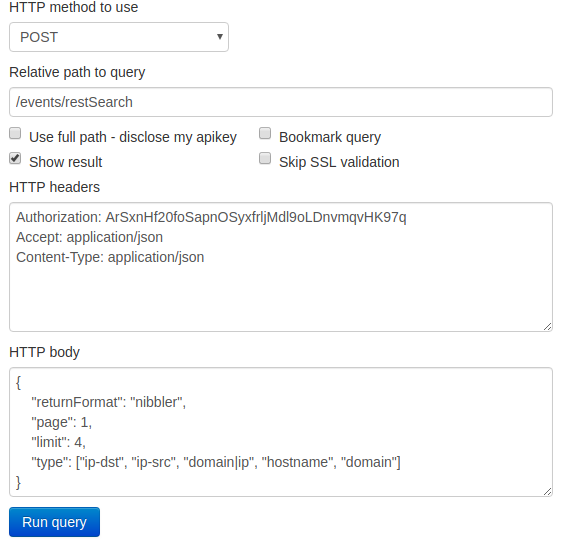
\includegraphics[scale=0.5]{nibbler_rest_client.png}
  \end{center}
\end{frame}


